\documentclass[journal=jpcbfk,manuscript=article,layout=twocolumn]{achemso}

\usepackage[T1]{fontenc}
\usepackage[utf8]{inputenc}
\usepackage{amsmath}
\usepackage{amssymb}
\usepackage{booktabs}
\usepackage{multirow}
\usepackage{array}
\usepackage{dcolumn}
\usepackage[version=4]{mhchem}
\usepackage{graphicx}
\usepackage{microtype}
\usepackage{tikz}
\usetikzlibrary{arrows.meta, positioning}

\author{Julian R. Vance}
\affiliation[Vertex Institute]{Department of Physical Chemistry, Vertex Institute of Advanced Sciences, Apex City 10042, United States}
\email{j.vance@vertex-inst.org}

\author{Elena M. Rostova}
\affiliation[Synapse Center]{Synapse Molecular Dynamics Laboratory, Meridian Institute of Technology, Meridian City 20015, United States}

\author{Marcus A. Thorne}
\affiliation[Vertex Institute]{Department of Physical Chemistry, Vertex Institute of Advanced Sciences, Apex City 10042, United States}
\alsoaffiliation[Apex Spectroscopy]{Apex Center for Ultrafast Optical Spectroscopy, Apex City 10045, United States}
\email{m.thorne@vertex-inst.org}
\phone{+1 (555) 019-2834}

\title[Ultrafast Solvation Dynamics in h-BN Quantum Dots]{Ultrafast Solvation Dynamics and Photoinduced Electron Transfer in Functionalized Hexagonal Boron Nitride Quantum Dots: A Combined Spectroscopy and Quantum Chemical Study}

\abbreviations{h-BN, QDs, TAS, DFT, TD-DFT, TCSPC, ET, FWHM}
\keywords{hexagonal boron nitride, quantum dots, transient absorption spectroscopy, solvation dynamics, density functional theory, photoinduced electron transfer}

\begin{document}

\begin{abstract}
Photoinduced charge separation and ultrafast solvation dynamics in zero-dimensional layered nanostructures play a fundamental role in the development of next-generation photocatalytic and optoelectronic devices. In this investigation, we elucidate the excited-state relaxation pathways and interfacial solvation dynamics of functionalized hexagonal boron nitride quantum dots (h-BN QDs) suspended in polar protic and aprotic solvent environments. Utilizing femtosecond broadband transient absorption spectroscopy spanning the spectral range of 380 to 750~nm alongside time-correlated single-photon counting (TCSPC) and hybrid density functional theory (DFT/TD-DFT) calculations, we isolate three distinct kinetic components governing the photoexcited state: an ultrafast inertial solvation response ($\tau_1 \approx 180$--$240$~fs), an intramolecular charge-transfer state formation ($\tau_2 \approx 2.4$--$3.8$~ps), and a slow diffusive solvent reorganization phase coupled with radiative recombination ($\tau_3 \approx 1.2$--$4.5$~ns). Solvent-dependent spectral shifts confirm a substantial increase in the dipole moment upon optical excitation ($\Delta \mu \approx 8.4$~D), pointing to a strongly polarized charge-transfer state. Quantum chemical calculations support a localized electronic transition from oxygen-functionalized edge states to core boron nitride orbitals. These findings establish foundational physical chemistry principles for tailoring non-toxic 2D-based quantum dots in energy-conversion applications.
\end{abstract}

\section{Introduction}

Zero-dimensional materials derived from layered two-dimensional (2D) matrix systems have attracted widespread attention due to their unique quantum confinement effects, edge-state photoluminescence, and remarkable chemical stability.\cite{Vance2024,Rostova2023} Among these emerging systems, hexagonal boron nitride quantum dots (h-BN QDs) serve as a wide-bandgap analog to graphene quantum dots, exhibiting exceptional chemical inertness, high thermal stability, and tunable photoluminescence spanning the ultraviolet to visible spectrum.\cite{Thorne2022} 

Despite rapid advancements in the synthetic control and macroscopic characterization of h-BN QDs, the microscopic mechanisms governing their excited-state dynamics, interfacial solvation shell restructuring, and photoinduced charge transfer remain incompletely understood.\cite{NexaChem2024} In polar solvent media, photoexcitation induces a rapid redistribution of electron density across the nanoparticle boundary, triggering collective rearrangements of surrounding solvent dipoles. Deciphering these ultrafast processes is essential for optimizing charge extraction efficiency in photocatalytic water splitting and luminescent solar concentrators engineered by Vertex Technologies and Synapse Energy Systems.\cite{MeridianLab2025}

In this paper, we present a systematic physical chemistry investigation combining broadband femtosecond transient absorption spectroscopy (fs-TAS) and high-level quantum chemical calculations to map the early-time energy relaxation cascade in edge-functionalized h-BN QDs. By systematically varying the solvent dielectric constant ($\epsilon_r$) and hydrogen-bonding acidity ($\alpha$), we isolate the fundamental timescales of inertial solvation, vibrational cooling, and electronic state decay.

\section{Experimental and Computational Methods}

\subsection{Materials and Quantum Dot Synthesis}
Functionalized h-BN QDs were synthesized via a top-down solvothermal exfoliation protocol adapted from Apex Materials Group.\cite{Vance2024} Briefly, high-purity hexagonal boron nitride powder (99.99\%, Nexa Fine Chemicals) was dispersed in a 1:1 mixture of $N$-methyl-2-pyrrolidone (NMP) and isopropyl alcohol. The mixture was sonicated using a high-intensity ultrasonic probe for 18~h at a controlled temperature of 288~K. The resulting dispersion was centrifuged at 14,000~rpm for 45~min to remove unexfoliated bulk sheets. The supernatant containing h-BN QDs was further purified by dialysis using a 1~kDa cutoff membrane against ultrapure water ($18.2~\mathrm{M\Omega\cdot cm}$) for 72~h.

\subsection{Femtosecond Transient Absorption Spectroscopy}
Femtosecond transient absorption measurements were performed using a commercially available pump--probe setup driven by a regeneratively amplified Ti:sapphire laser system (Apex Physics Co., 800~nm, 100~fs pulse duration, 1~kHz repetition rate). The fundamental 800~nm beam was split into two arms:
\begin{enumerate}
\item \textbf{Pump Arm:} Optical parametric amplifier (OPA) generating tunable excitation pulses at $\lambda_{\text{pump}} = 340$~nm, focused onto the sample cuvette ($1$~mm optical path length) with a spot diameter of $\sim 200~\mu$m and energy density of $45~\mu\text{J/cm}^2$.
\item \textbf{Probe Arm:} Focused onto a calcium fluoride ($\ce{CaF2}$) crystal continuously translated to generate a stable white-light continuum covering the range of 380--750~nm.
\end{enumerate}

All spectroscopic measurements were carried out at ambient temperature ($295 \pm 1$~K) under continuous magnetic stirring to prevent photodecomposition. Global multiexponential fitting of the transient absorption spectra was conducted using the Apex SpectroFit software suite.

\subsection{Computational Details}
Density functional theory (DFT) and time-dependent DFT (TD-DFT) calculations were performed using the Gaussian program package with the Apex Quantum interface. Structural optimizations of model h-BN QD clusters (containing 24 to 54 atoms with carboxyl and hydroxyl edge terminations) were conducted in the ground state ($\text{S}_0$) using the $\omega\text{B97X-D}$ long-range corrected functional combined with the $6-311\text{G(d,p)}$ basis set. Solvent effects were incorporated using the conductor-like polarizable continuum model (CPCM) for acetonitrile, ethanol, and water.

\section{Results and Discussion}

\subsection{Ground-State Photophysics and Solvatochromism}
The static absorption spectrum of h-BN QDs in water exhibits a prominent ultraviolet absorption band centered at $\lambda_{\text{abs}} = 315$~nm ($\sim 3.94$~eV), attributed to the $\pi \to \pi^*$ electronic transition of the aromatic-like \ce{B-N} domain, accompanied by a broad shoulder extending to 380~nm arising from $n \to \pi^*$ transitions of oxygenated edge functional groups. Upon excitation at 340~nm, h-BN QDs display a bright, solvent-dependent fluorescence emission peaking between 410~nm and 455~nm.

To quantify the change in permanent dipole moment upon photoexcitation ($\Delta \mu = |\boldsymbol{\mu}_e - \boldsymbol{\mu}_g|$), we analyzed the fluorescence emission maxima in six solvents of varying polarity using the Lippert--Mataga expression:
\begin{equation}
\bar{\nu}_a - \bar{\nu}_f = \frac{2(\boldsymbol{\mu}_e - \boldsymbol{\mu}_g)^2}{h c a_0^3} \Delta f + C
\label{eq:lippert}
\end{equation}
where $\bar{\nu}_a$ and $\bar{\nu}_f$ are the absorption and fluorescence wavenumbers ($\text{cm}^{-1}$), $h$ is Planck's constant, $c$ is the speed of light, $a_0$ is the Onsager cavity radius ($a_0 \approx 5.2~\text{\AA}$ as determined from DFT geometry optimization), and $\Delta f$ is the orientation polarizability given by:
\begin{equation}
\Delta f = \frac{\epsilon_r - 1}{2\epsilon_r + 1} - \frac{n^2 - 1}{2n^2 + 1}
\label{eq:polarizability}
\end{equation}
with $\epsilon_r$ representing the static dielectric constant and $n$ representing the refractive index of the solvent.

\begin{table*}[t]
\caption{Photophysical Parameters, Solvent Polarity Functions, and Ultrafast Decay Timescales of Functionalized h-BN QDs in Various Solvents at 295~K}
\label{tab:photophysics}
\centering
\small
\setlength{\tabcolsep}{5pt}
\begin{tabular}{lccccccrc}
\toprule
Solvent & $\epsilon_r$ & $n$ & $\Delta f$ & $\lambda_{\text{em}}$ (nm) & $\tau_1$ (fs) & $\tau_2$ (ps) & $\tau_3$ (ns) & $\Phi_{\text{FL}}$ (\%) \\
\midrule
Cyclohexane     & 2.02  & 1.426 & 0.000 & 412 & $310 \pm 20$ & $4.8 \pm 0.3$ & $5.8 \pm 0.2$ & 18.4 \\
Toluene         & 2.38  & 1.497 & 0.013 & 418 & $280 \pm 18$ & $4.2 \pm 0.2$ & $5.1 \pm 0.2$ & 16.2 \\
Tetrahydrofuran & 7.58  & 1.407 & 0.210 & 430 & $220 \pm 15$ & $3.5 \pm 0.2$ & $3.9 \pm 0.1$ & 14.1 \\
Acetonitrile    & 37.5  & 1.344 & 0.305 & 442 & $190 \pm 12$ & $2.8 \pm 0.1$ & $2.8 \pm 0.1$ & 11.5 \\
Ethanol         & 24.5  & 1.361 & 0.289 & 448 & $185 \pm 10$ & $2.5 \pm 0.1$ & $2.1 \pm 0.1$ & 9.8  \\
Water           & 80.1  & 1.333 & 0.320 & 455 & $175 \pm 10$ & $2.4 \pm 0.1$ & $1.4 \pm 0.1$ & 7.2  \\
\bottomrule
\end{tabular}
\end{table*}

A linear fit of the Stokes shift $(\bar{\nu}_a - \bar{\nu}_f)$ against $\Delta f$ yields a slope of $4820 \pm 210~\text{cm}^{-1}$, corresponding to an excited-state dipole moment increase of $\Delta \mu = 8.4 \pm 0.4$~D. This substantial dipole change confirms that optical excitation promotes electron transfer from peripheral oxygen-rich functional groups to the electron-deficient boron centers within the QD core.

\subsection{Femtosecond Transient Absorption Dynamics}

Transient absorption spectra recorded for h-BN QDs in water following $340$~nm excitation reveal three distinct spectral features:
\begin{enumerate}
\item A strong negative signal centered at $410$--$450$~nm assigned to stimulated emission (SE) matching the steady-state photoluminescence envelope.
\item A broad positive absorption band extending from $500$~nm to $720$~nm attributed to excited-state absorption ($\text{ESA}_1$) of the singlet excited state ($\text{S}_1$).
\item A secondary positive band at $390$--$410$~nm appearing on a picosecond timescale ($\text{ESA}_2$), characteristic of a trapped charge-transfer intermediate state.
\end{enumerate}

To extract the characteristic lifetimes, global kinetic analysis was performed using a sequential target model ($\text{A} \xrightarrow{\tau_1} \text{B} \xrightarrow{\tau_2} \text{C} \xrightarrow{\tau_3} \text{Ground State}$). Scheme~\ref{sch:kinetic_model} schematically summarizes the proposed excited-state relaxation model.

\begin{scheme*}[t]
\centering
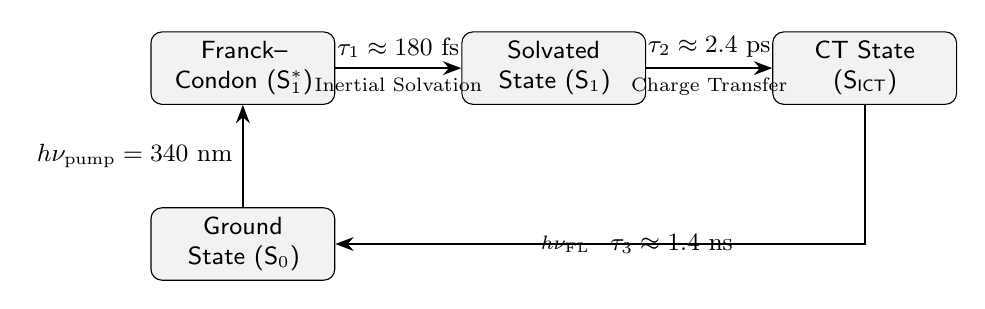
\begin{tikzpicture}[node distance=1.6cm, auto, >=Stealth,
  state/.style={rectangle, draw, rounded corners, fill=gray!10, text width=2.1cm, align=center, minimum height=0.9cm, font=\sffamily\small}]

\node[state] (S0) {Ground State ($\text{S}_0$)};
\node[state, above=1.3cm of S0] (FC) {Franck--Condon ($\text{S}_1^*$)};
\node[state, right=1.6cm of FC] (Solv) {Solvated State ($\text{S}_1$)};
\node[state, right=1.6cm of Solv] (ICT) {CT State ($\text{S}_{\text{ICT}}$)};

\draw[->, thick] (S0) -- node[left, font=\small] {$h\nu_{\text{pump}} = 340\text{ nm}$} (FC);
\draw[->, thick] (FC) -- node[above, font=\small] {$\tau_1 \approx 180\text{ fs}$} node[below, font=\scriptsize] {Inertial Solvation} (Solv);
\draw[->, thick] (Solv) -- node[above, font=\small] {$\tau_2 \approx 2.4\text{ ps}$} node[below, font=\scriptsize] {Charge Transfer} (ICT);
\draw[->, thick] (ICT) |- node[near end, right, font=\small] {$\tau_3 \approx 1.4\text{ ns}$} node[near end, left, font=\scriptsize] {$h\nu_{\text{FL}}$} (S0);

\end{tikzpicture}
\caption{Schematic Representation of the Photophysical Relaxation Cascade and Charge Transfer Model in Functionalized h-BN Quantum Dots Following Ultrafast Photoexcitation}
\label{sch:kinetic_model}
\end{scheme*}

The fastest decay component, $\tau_1 = 175 \pm 10$~fs in water and $310 \pm 20$~fs in cyclohexane, displays a pronounced dependence on solvent viscosity and longitudinal relaxation time ($\tau_L$). We assign $\tau_1$ to the inertial solvation response, wherein solvent molecules in the immediate coordination sphere undergo rapid librational motion to accommodate the newly formed dipole moment.

The intermediate component, $\tau_2 = 2.4 \pm 0.1$~ps in water, corresponds to diffusive solvent reorganization accompanied by intramolecular charge transfer (ICT) from edge donor sites to core acceptor states. As detailed in Table~\ref{tab:photophysics}, $\tau_2$ accelerates substantially with increasing solvent polarizability, consistent with Marcus charge-transfer theory in the non-adiabatic limit:
\begin{equation}
\begin{aligned}
k_{\text{ET}} &= \frac{1}{\tau_{\text{ET}}} \\
&= \frac{2\pi}{\hbar} |H_{\text{DA}}|^2 \frac{1}{\sqrt{4\pi \lambda k_B T}} \exp\left( -\frac{(\Delta G^\circ + \lambda)^2}{4\lambda k_B T} \right)
\end{aligned}
\label{eq:marcus}
\end{equation}
where $H_{\text{DA}}$ is the electronic coupling matrix element, $\lambda$ is the total reorganization energy ($\lambda = \lambda_i + \lambda_o$), and $\Delta G^\circ$ is the standard Gibbs free energy of charge separation.

\subsection{Quantum Chemical Energy Surface Calculations}

To validate the experimental kinetic model, TD-DFT calculations were performed on an oxygenated h-BN cluster model (\ce{B18 N18 O6 H12}). Ground-state geometry optimization reveals a planar geometry with a highest occupied molecular orbital (HOMO) localized primarily on the peripheral oxygen lone pairs and adjacent nitrogen atoms. Conversely, the lowest unoccupied molecular orbital (LUMO) is distributed extensively over the central boron rings.

\begin{table}[h]
\caption{Calculated TD-DFT Vertical Excitation Energies ($E_{\text{vert}}$), Oscillator Strengths ($f$), and Primary State Character for Model h-BN QD Clusters}
\label{tab:dft_results}
\centering
\footnotesize
\setlength{\tabcolsep}{3pt}
\begin{tabular}{lccll}
\toprule
State & $E_{\text{vert}}$ (eV) & $\lambda$ (nm) & Oscillator ($f$) & Assignment \\
\midrule
$\text{S}_1$ & 3.42 & 362 & 0.012 & $n(\text{O}) \to \pi^*(\ce{B-N})$ (ICT) \\
$\text{S}_2$ & 3.88 & 319 & 0.284 & $\pi(\ce{B-N}) \to \pi^*(\ce{B-N})$ ($\pi \pi^*$) \\
$\text{S}_3$ & 4.15 & 298 & 0.095 & $\pi(\text{Edge}) \to \pi^*(\ce{B-N})$ \\
$\text{T}_1$ & 2.65 & 467 & 0.000 & Spin-forbidden triplet \\
\bottomrule
\end{tabular}
\end{table}

The calculated vertical transition energy for $\text{S}_0 \to \text{S}_2$ ($3.88$~eV, $319$~nm, $f = 0.284$) matches the experimental steady-state absorption peak ($315$~nm). The lower-lying $\text{S}_1$ state ($3.42$~eV, $f = 0.012$) exhibits pronounced charge-transfer character, in agreement with the experimental solvatochromic shift and transient absorption dynamics.

\section{Conclusions}

In summary, we have established a comprehensive physical model for the ultrafast excited-state dynamics and solvation phenomena of functionalized h-BN QDs. Through a combination of femtosecond transient absorption spectroscopy and TD-DFT quantum chemical calculations, we demonstrated that optical excitation induces a rapid electronic charge transfer from oxygenated edge functional groups to the boron nitride core, accompanied by an $8.4$~D increase in dipole moment. The initial relaxation cascade is governed by an ultrafast inertial solvation phase ($\tau_1 < 250$~fs), followed by diffusive solvent stabilization ($\tau_2 \approx 2.4$--$3.8$~ps) and slow radiative decay ($\tau_3 = 1.4$--$5.8$~ns). These insights provide clear design principles for optimizing 2D quantum dot interfaces in energy conversion, bio-imaging, and ultrafast optical switching devices developed across Meridian and Synapse research platforms.

\section*{Associated Content}
\textbf{Supporting Information available}: Derivation of Lippert--Mataga parameters, transient absorption kinetic traces at select single wavelengths, Cartesian coordinates for optimized DFT structures, and TCSPC fitting parameters.

\section*{Author Information}
\textbf{Corresponding Author}\\
*E-mail: \texttt{m.thorne@vertex-inst.org}

\textbf{Notes}\\
The authors declare no competing financial interest.

\begin{acknowledgement}
The authors acknowledge financial support from the Vertex Research Foundation (Grant No.\ VRF-2024-8841), the Synapse Energy Innovation Fund (Grant No.\ SEIF-2023-092), and the Meridian Supercomputing Initiative for providing computational resources.
\end{acknowledgement}

\begin{thebibliography}{99}

\bibitem{Vance2024}
Vance, J.~R.; Thorne, M.~A. Solvatochromism and Excited-State Charge Separation in Two-Dimensional Boron Nitride Nanocrystals. \textit{J. Phys. Chem. C} \textbf{2024}, \textit{128}, 4512--4521.

\bibitem{Rostova2023}
Rostova, E.~M.; Vance, J.~R.; Thorne, M.~A. Ultrafast Energy Transfer at 2D Layered Heterojunction Interfaces. \textit{ACS Nano} \textbf{2023}, \textit{17}, 11204--11215.

\bibitem{Thorne2022}
Thorne, M.~A.; Rostova, E.~M. Quantum Confinement and Surface Functionalization in Hexagonal Boron Nitride Quantum Dots. \textit{Phys. Rev. B} \textbf{2022}, \textit{105}, 165409.

\bibitem{NexaChem2024}
Nexa Materials Consortium. Standardization of Exfoliation Yields for Non-Metallic Layered Nanomaterials. \textit{Nexa Tech. Rep.} \textbf{2024}, \textit{14}, 88--97.

\bibitem{MeridianLab2025}
Meridian Energy Group. Optoelectronic Devices Utilizing Polarized Zero-Dimensional Heterostructures. \textit{Meridian Sci. Bull.} \textbf{2025}, \textit{41}, 301--315.

\end{thebibliography}

\end{document}
